\section{Sensitivities}
\label{sec:sens}

In this section, various sensitivity results are presented. For the sake of simplicity, unless otherwise stated, only true normal ordering is shown. Possible variations of sensitivity are presented in two ways. Results produced using Asimovs are shown as lines, and differences between two Asimov scenarios are shown with a colored band. Note that the band in the Asimov case is purely to guide the eye, and does not denote a confidence interval. For results produced using many throws of oscillation parameters, systematic and statistical uncertainties, $\sim$300,000 throws were used to calculate the sensitivity for each scenario. The median sensitivity is shown with a solid line, and a transparent filled area indicates the region containing the central 68\% of throws, which can be interpreted as the 1$\sigma$ uncertainty on the sensitivity.

\begin{figure}[htbp]
  \centering
  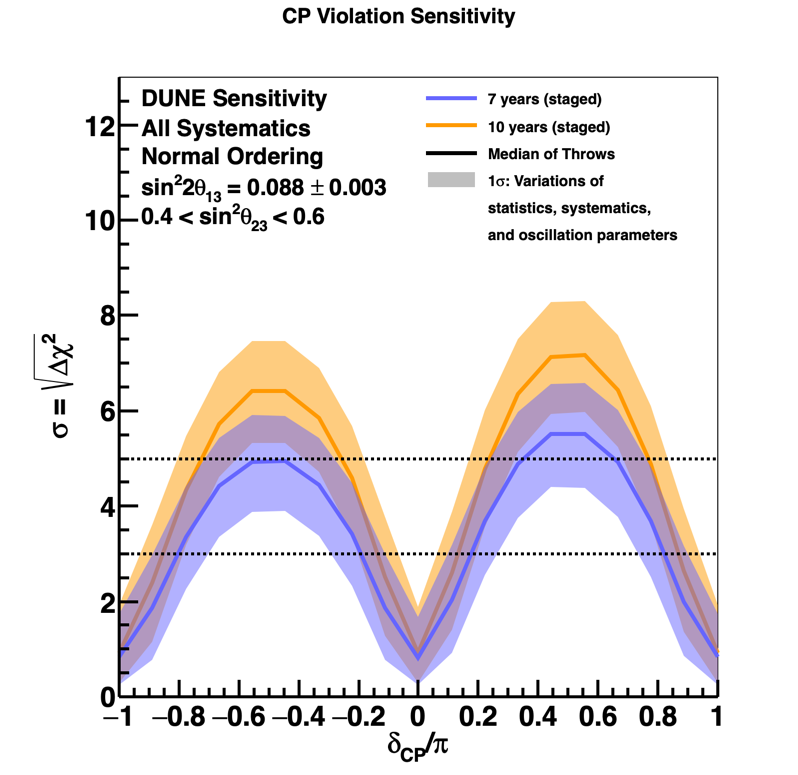
\includegraphics[width=0.98\linewidth, trim={0cm 0cm 0cm 2.3cm}, clip]{cpv_two_exps_throws_nh_2019_v4.png}\\
  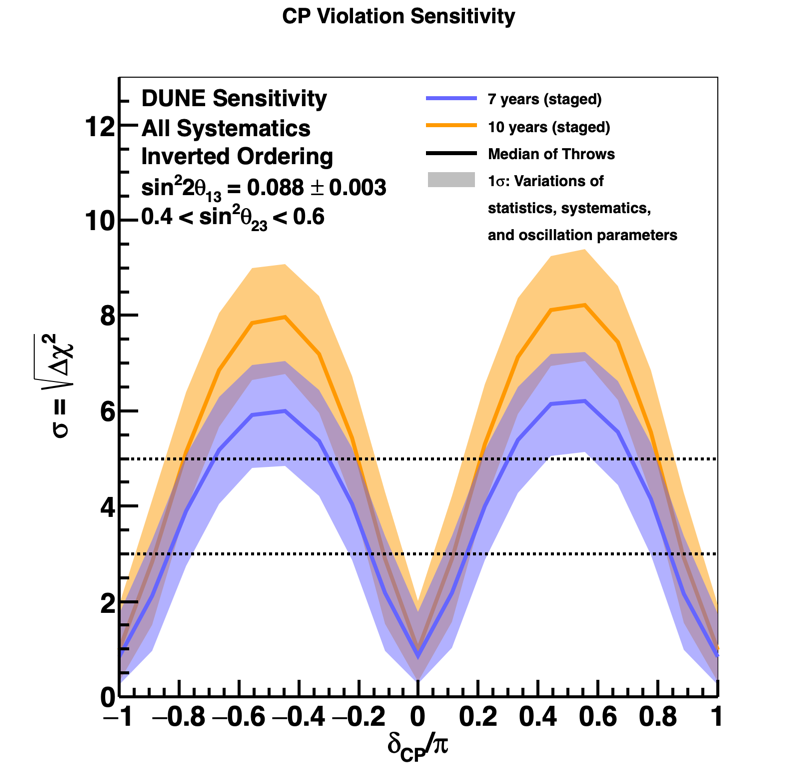
\includegraphics[width=0.98\linewidth, trim={0cm 0cm 0cm 2.3cm}, clip]{cpv_two_exps_throws_ih_2019_v4.png}
  \caption[Significance of the DUNE determination of CP-violation as a function of \deltacp in both \dword{no} and \dword{io}]{Significance of the DUNE determination of CP-violation ($\deltacp \neq [0,\pm\pi]$) as a function of the true value of \deltacp, for seven (blue) and ten (orange) years of exposure, in both normal (top) and inverted (bottom) ordering. The width of the transparent bands cover 68\% of fits in which random throws are used to simulate statistical variations and select true values of the oscillation and systematic uncertainty parameters, constrained by pre-fit uncertainties. The solid lines show the median sensitivity.}
  \label{fig:cpv_nominal}
\end{figure}
Figure~\ref{fig:cpv_nominal} shows the significance with which \dword{cpv} ($\deltacp \neq [0, \pm\pi]$) can be observed in both \dword{no} and \dword{io} as a
function of the true value of \deltacp for exposures corresponding to seven and ten years of data, using the staging scenario described in Section~\ref{sec:rate}, and using the toy throwing method described in Section~\ref{sec:methods} to investigate their effect on the sensitivity.
This sensitivity has a characteristic double peak
structure because the significance of a \dword{cpv} measurement
necessarily decreases around CP-conserving values of \deltacp.
The median \dword{cpv} sensitivity reaches 5$\sigma$ for a small range of values after an exposure of seven years in \dword{no}, and a broad range of values after a ten year exposure. In \dword{io}, \dword{dune} has slightly stronger sensitivity to \dword{cpv}, and reaches 5$\sigma$ for a broad range of values after a seven year exposure.
Note that with statistical and systematic throws, the median sensitivity never reaches exactly zero.

\begin{figure}[htbp]
    \centering
    \includegraphics[width=0.98\linewidth, trim={0cm 0cm 0cm 2.3cm}, clip]{cpv_varyth23_2019_v4.png}\\
    \includegraphics[width=0.98\linewidth, trim={0cm 0cm 0cm 2.3cm}, clip]{cpv_varyth13_2019_v4.png}\\
    \includegraphics[width=0.98\linewidth, trim={0cm 0cm 0cm 2.3cm}, clip]{cpv_varydmsq_2019_v4.png}    
    \caption{Asimov sensitivity to CP violation, as a function of the true value of $\deltacp$, for ten years of exposure. Curves are shown for variations in the true values of $\theta_{23}$ (top), $\theta_{13}$ (middle) and $\Delta m^2_{32}$ (bottom), which correspond to their 3$\sigma$ \dword{nufit} range of values, as well as the \dword{nufit} central value, and maximal mixing.}
    \label{fig:cpv_oa_var}
\end{figure}
Figure~\ref{fig:cpv_oa_var} shows the \dword{dune} Asimov sensitivity to \dword{cpv} in \dword{no} when the true values of $\theta_{23}$, $\theta_{13}$, and $\Delta m^{2}_{32}$ vary within the 3$\sigma$ range allowed by \dword{nufit}. The largest effect is the variation in sensitivity with the true value of $\theta_{23}$, where degeneracy with $\deltacp$ and matter effects are significant. Values of $\theta_{23}$ in the lower octant lead to the best sensitivity to \dword{cpv}. The true values of $\theta_{13}$ and $\Delta m^2_{32}$ are highly constrained by global data and, within these constraints, do not have a dramatic impact on the sensitivity.
Note that in the Asimov cases shown in Figure~\ref{fig:cpv_oa_var}, the median sensitivity reaches 0 at \dword{cp}-conserving values of \deltacp (unlike the case with the throws as in Figure~\ref{fig:cpv_nominal}), but in regions far from \dword{cp}-conserving values, the Asimov sensitivity and the median sensitivity from the throws agree well.


\begin{figure}[htbp]
  \centering
  \includegraphics[width=0.98\linewidth, trim={0cm 0cm 0cm 2.3cm}, clip]{cpv_exp_varyconstr_nh_2019_v4.png}
  \includegraphics[width=0.98\linewidth, trim={0cm 0cm 0cm 2.3cm}, clip]{cpv_exp_varyth23_nh_2019_v4.png}
  \caption[Significance of the DUNE determination of CP-violation as a function of exposure]{Significance of the DUNE determination of CP-violation ($\deltacp \neq [0,\pi]$) for the case when \deltacp=$-\pi/2$, and for 50\% and 75\% of possible true \deltacp values, as a function of exposure in kt-MW-years. Top: The width of the band shows the impact of applying an external constraint on $\theta_{13}$. Bottom: The width of the band shows the impact of varying the true value of \sinst{23} within the \dword{nufit} 90\% C.L. region.}
  \label{fig:cpv_exposure}
\end{figure}
Figure~\ref{fig:cpv_exposure} shows the result of Asimov studies investigating the significance
with which \dword{cpv} can be determined in \dword{no} for 75\% and 50\% of \deltacp values, and when $\deltacp=-\pi/2$, as a function of exposure in kt-MW-years, which can be converted to years using the staging scenario described in Section~\ref{sec:rate}. The width of the bands show the impact of applying an external constraint on $\theta_{13}$. CP violation can be observed with 5$\sigma$ significance after about seven years (336 kt-MW-years) if \deltacp = $-\pi/2$ and after about ten years (624 kt-MW-years) for 50\% of \deltacp values. CP violation can be observed with 3$\sigma$ significance for 75\% of \deltacp values after about 13 years of running. In the bottom plot of Figure~\ref{fig:cpv_exposure}, the width of the bands shows the impact of applying an external constraint on $\theta_{13}$, while in the bottom plot, the width of the bands is the result of varying the true value of \sinst{23} within the \dword{nufit} 90\% C.L. allowed region.

\begin{figure}[htbp]
  \centering
  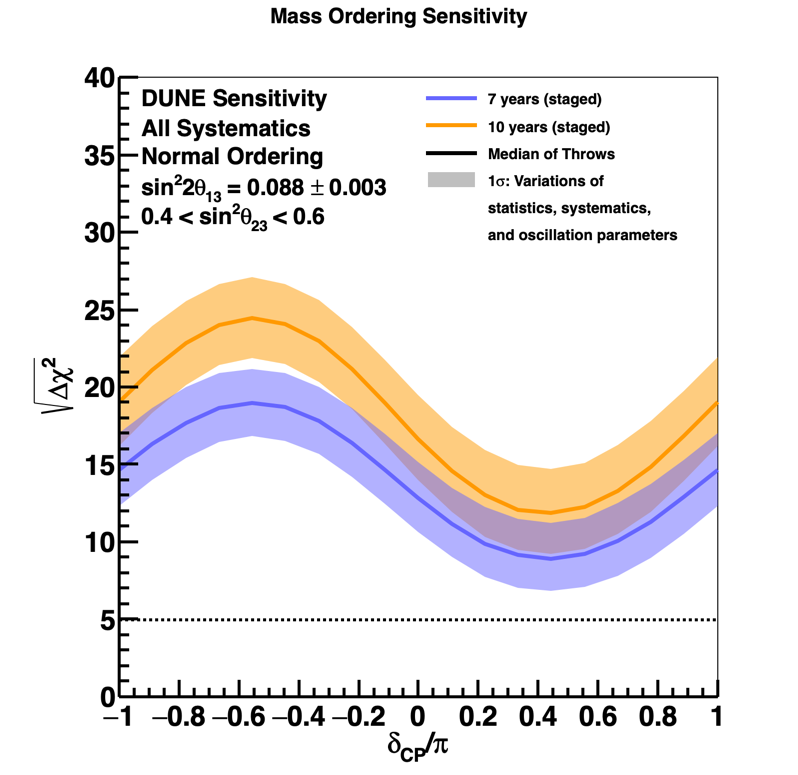
\includegraphics[width=0.98\linewidth, trim={0cm 0cm 0cm 2.3cm}, clip]{mh_two_exps_throws_nh_2019_v4.png}
  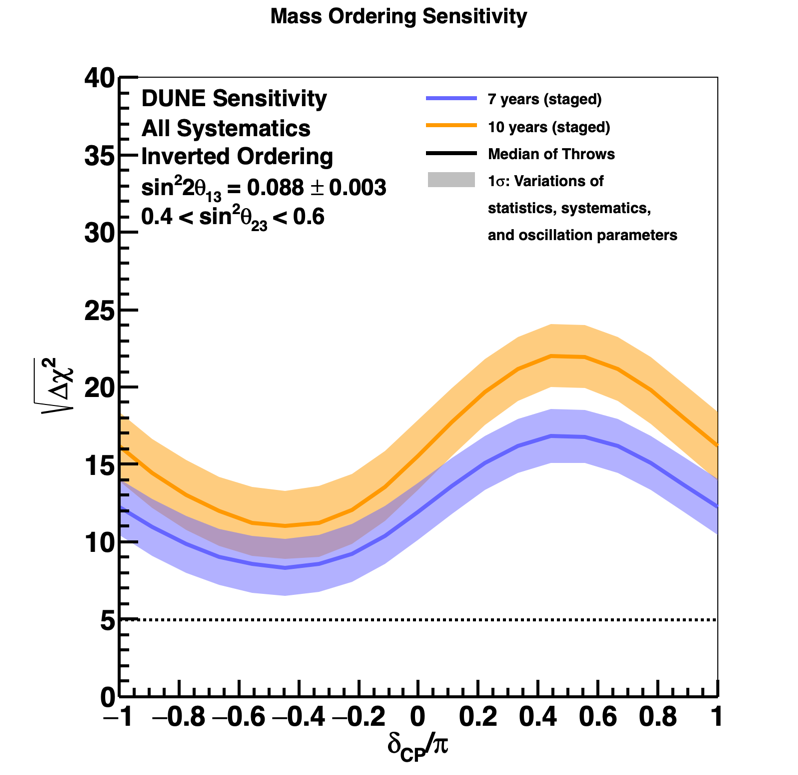
\includegraphics[width=0.98\linewidth, trim={0cm 0cm 0cm 2.3cm}, clip]{mh_two_exps_throws_ih_2019_v4.png}
  \caption[Significance of the DUNE neutrino mass ordering determination, as a function of \deltacp]{Significance of the DUNE determination of the neutrino mass ordering, as a function of the true value of \deltacp, for seven (blue) and ten (orange) years of exposure. The width of the transparent bands cover 68\% of fits in which random throws are used to simulate statistical variations and select true values of the oscillation and systematic uncertainty parameters, constrained by pre-fit uncertainties. The solid lines show the median sensitivity.}
  \label{fig:mh_nominal}
\end{figure}
Figure~\ref{fig:mh_nominal} shows the significance with which the neutrino mass ordering can be determined in both \dword{no} and \dword{io} as a function of the true value of \deltacp, for both seven and ten year exposures, including the effect of all other oscillation and systematic parameters using the toy throwing method described in Section~\ref{sec:methods}. The characteristic shape results from near degeneracy between matter and \dword{cpv} effects that occurs near $\deltacp=\pi/2$ ($-\deltacp=\pi/2$) for true normal (inverted) ordering. Studies have indicated that special attention must be paid to the statistical interpretation of neutrino mass ordering sensitivities~\cite{Ciuffoli:2013rza,Qian:2012zn,Blennow:2013oma} because the $\Delta\chi^2$ metric does not follow the expected chi-square function for one degree of freedom, so the interpretation of the $\sqrt{\Delta \chi^{2}}$ as the sensitivity is complicated. However, it is clear from Figure~\ref{fig:mh_nominal} that \dword{dune} is able to distinguish the mass ordering for both true \dword{no} and \dword{io}, and using the corrections from, for example, Ref.~\cite{Ciuffoli:2013rza}, DUNE would still achieve 5$\sigma$ significance for the central 68\% of all throws shown in Figure~\ref{fig:mh_nominal}. We note that for both seven and ten years (it was not checked for lower exposures), there were no parameter throws used in generating the plots ($\sim$300,000 each) for which the incorrect mass ordering was preferred.

\begin{figure}[htbp]
    \centering
    \includegraphics[width=0.98\linewidth, trim={0cm 0cm 0cm 2.3cm}, clip]{mh_varyth23_2019_v4.png}
    \includegraphics[width=0.98\linewidth, trim={0cm 0cm 0cm 2.3cm}, clip]{mh_varyth13_2019_v4.png}
    \includegraphics[width=0.98\linewidth, trim={0cm 0cm 0cm 2.3cm}, clip]{mh_varydmsq_2019_v4.png}
    \caption{Asimov sensitivity to the neutrino mass ordering, as a function of the true value of $\deltacp$, for ten years of exposure. Curves are shown for variations in the true values of $\theta_{23}$ (top), $\theta_{13}$ (middle) and $\Delta m^2_{32}$ (bottom), which correspond to their 3$\sigma$ \dword{nufit} range of values, as well as the \dword{nufit} central value. and maximal mixing.}
    \label{fig:mh_oa_var}
\end{figure}
Figure~\ref{fig:mh_oa_var} shows the \dword{dune} Asimov sensitivity to the neutrino mass ordering when the true values of $\theta_{23}$, $\theta_{13}$, and $\Delta m^{2}_{32}$ vary within the 3$\sigma$ range allowed by \dword{nufit}. As for \dword{cpv} (in Figure~\ref{fig:cpv_oa_var}), the largest variation in sensitivity is with the true value of $\theta_{23}$, but in this case, the upper octant leads to the best sensitivity. Again, the true values of $\theta_{13}$ and $\Delta m^2_{32}$ do not have a dramatic impact on the sensitivity. The median Asimov sensitivity tracks the median throws shown in Figure~\ref{fig:mh_nominal} well for the reasonably high exposures tested --- this was not checked for exposures below seven years (336 kt-MW-years).

\begin{figure}[htbp]
    \centering
    \includegraphics[width=0.98\linewidth, trim={0cm 0cm 0cm 2.3cm}, clip]{mh_exp_varyconstr_nh_2019_v4.png}\\
    \includegraphics[width=0.98\linewidth, trim={0cm 0cm 0cm 2.3cm}, clip]{mh_exp_varyth23_nh_2019_v4.png} 
    \caption[Significance of the DUNE neutrino mass ordering determination as a function of exposure]{Significance of the DUNE determination of the neutrino mass ordering for the case when \deltacp=$-\pi/2$, and for 100\% of possible true \deltacp values, as a function of exposure in kt-MW-years. Top: The width of the band shows the impact of applying an external constraint on $\theta_{13}$. Bottom: The width of the band shows the impact of varying the true value of \sinst{23} within the \dword{nufit} 90\% C.L. region.}
    \label{fig:mh_exposure}
\end{figure}
Figure~\ref{fig:mh_exposure} shows the result of Asimov studies assessing the significance
with which the neutrino mass ordering can be determined for 100\% of \deltacp values, and when $\deltacp=-\pi/2$, as a function of exposure in kt-MW-years, for true \dword{no}. The width of the bands show the impact of applying an external constraint on $\theta_{13}$. The bottom plot shows the impact of varying the true value of \sinst{23} within the \dword{nufit} 90\% C.L. region. As DUNE will be able to establish the neutrino mass ordering at the 5$\sigma$ level for 100\% of \deltacp values after a relatively short period, these plots only extend to 500 kt-MW-years. 

\begin{figure}[htbp]
  \centering
  \includegraphics[width=0.98\linewidth]{octant_no_2019_v4.png}\\
  \includegraphics[width=0.98\linewidth]{octant_io_2019_v4.png}
  \caption[Sensitivity of determination of the $\theta_{23}$ octant as a function of \sinst{23} in both \dword{no} and \dword{io}]{Sensitivity to determination of the $\theta_{23}$ octant as a function of the true value of \sinst{23}, for ten (orange) and fifteen (green) years of exposure, for both normal (top) and inverted (bottom) ordering. The width of the transparent bands cover 68\% of fits in which random throws are used to simulate statistical variations and select true values of the oscillation and systematic uncertainty parameters, constrained by pre-fit uncertainties. The solid lines show the median sensitivity.}
    \label{fig:lbloctant}
\end{figure}
The measurement of $\nu_\mu \rightarrow \nu_\mu$ oscillations depends on $\sin ^2 2 \theta_{23}$, whereas the measurement of $\nu_\mu \rightarrow \nu_e$ oscillations depends on $\sin^2 \theta_{23}$.  A combination of both $\nu_e$ appearance and $\nu_\mu$ disappearance measurements can probe both maximal mixing and
the $\theta_{23}$ octant.  
Figure~\ref{fig:lbloctant} shows the sensitivity to determining the octant as a function of the true value of $\sinst{23}$, in both \dword{no} and \dword{io}. We note that the octant sensitivity strongly depends on the use of the external $\theta_{13}$ constraint.

In addition to the discovery potential for neutrino the mass ordering and \dword{cpv}, and sensitivity to the $\theta_{23}$ octant,  
\dword{dune} will improve the precision on key parameters that govern neutrino oscillations, including \deltacp, $\sin^22\theta_{13}$, \dm{31}, and $\sin^2\theta_{23}$.

\begin{figure}[htbp]
    \centering
    \includegraphics[width=0.98\linewidth]{dcpresvdcp_smooth_v4.png}
    \caption[Resolution for the DUNE measurement of \deltacp as a function of \deltacp]
	    {Resolution in degrees for the DUNE measurement of \deltacp, as a function of the true value of \deltacp, for seven (blue), ten (orange), and fifteen (green) years of exposure. The width of the band shows the impact of applying an external constraint on $\theta_{13}$.}
    \label{fig:dcpresvdcp}
\end{figure}
Figure~\ref{fig:dcpresvdcp} shows the resolution, in degrees, of DUNE's measurement of \deltacp, as a function of the true value of \deltacp, for true \dword{no}. The resolution on a parameter is produced from the central 68\% of post-fit parameter values using many throws of the systematic and remaining oscillation parameters, and statistical throws. The resolution of this measurement is significantly better near CP-conserving values of \deltacp, compared to maximally CP-violating values. For fifteen years of exposure, resolutions between 5$^{\circ}$--15$^{\circ}$ are possible, depending on the true value of \deltacp. A smoothing algorithm has been applied to interpolate between values of \deltacp at which the full analysis has been performed.

\begin{figure}[htbp]
    \centering
    \includegraphics[width=0.98\linewidth]{dcpres_exp_varyconstr_nh_2019_v4.png}\\
    \includegraphics[width=0.98\linewidth]{th13res_exp_varyconstr_nh_2019_v4.png} 
    \caption[Resolution of DUNE measurements of \deltacp and \sinstt{13}, as a function of exposure]{Resolution of DUNE measurements of \deltacp (top) and \sinstt{13} (bottom), as a function of exposure in kt-MW-years. As seen in Figure~\ref{fig:dcpresvdcp}, the \deltacp resolution has a significant dependence on the true value of \deltacp, so curves for $\deltacp=-\pi/2$ (red) and $\deltacp=0$ (green) are shown. For \deltacp, the width of the band shows the impact of applying an external constraint on $\theta_{13}$. No constraint is applied when calculating the \sinstt{13} resolution.}
    \label{fig:appres_exp}
\end{figure}
\begin{figure}[htbp]
    \centering
    \includegraphics[width=0.98\linewidth]{th23res_exp_varyconstr_nh_2019_v4.png}\\
    \includegraphics[width=0.98\linewidth]{dmsqres_exp_varyconstr_nh_2019_v4.png} 
    \caption[Resolution of DUNE measurements of \sinstt{23} (top) and $\Delta m^{2}_{32}$, as a function of exposure]{Resolution of DUNE measurements of \sinstt{23} (top) and $\Delta m^{2}_{32}$ (bottom), as a function of exposure in kt-MW-years. The width of the band for the \sinstt{23} resolution shows the impact of applying an external constraint on $\theta_{13}$. For the $\Delta m^{2}_{32}$ resolution, an external constraint does not have a significant impact, so only the unconstrained curve is shown.}
    \label{fig:disres_exp}
\end{figure}
Figures \ref{fig:appres_exp} and \ref{fig:disres_exp} show the resolution of DUNE's measurements of \deltacp and \sinstt{13} and of \sinstt{23} and $\Delta m^{2}_{32}$, respectively, as a function of exposure in kt-MW-years. The resolution on a parameter is produced from the central 68\% of post-fit parameter values using many throws of the systematic other oscillation parameters, and statistical throws. As seen in Figure~\ref{fig:dcpresvdcp}, the \deltacp resolution varies significantly with the true value of \deltacp, but for favorable values, resolutions near five degrees are possible for large exposure. The DUNE measurement of \sinstt{13} approaches the precision of reactor experiments for high exposure, allowing a comparison between the two results, which is of interest as a test of the unitarity of the PMNS matrix. 

\begin{figure}[htbp]
  \centering
  \includegraphics[width=0.98\linewidth]{bubbles_q13_2019_v4_allislands.png}
  \includegraphics[width=0.98\linewidth]{bubbles_atm_nopen_2019_v4.png}
  \caption[Two-dimensional 90\% constant $\Delta\chi^{2}$ confidence region in the \sinstt{13}--\deltacp and \sinst{23}--\dm{32} planes]{Two-dimensional 90\% constant $\Delta\chi^{2}$ confidence regions in the \sinstt{13}--\deltacp (top) and \sinst{23}--\dm{32} (botton) planes, for seven, ten, and fifteen years of exposure, with equal running in neutrino and antineutrino mode. The 90\% C.L. region for the \dword{nufit} global fit is shown in yellow for comparison. The true values of the oscillation parameters are assumed to be the central values of the \dword{nufit} global fit and the oscillation parameters governing long-baseline oscillation are unconstrained.}
    \label{fig:res_nopen_asimov0}
\end{figure}
\begin{figure}[htbp]
    \centering
    \includegraphics[width=0.98\linewidth]{bubbles_q23_asimov0_2019_v4.png}
    \caption[Two-dimensional 90\% constant $\Delta\chi^{2}$ confidence regions in the \sinst{23}--\deltacp plane]{Two-dimensional 90\% constant $\Delta\chi^{2}$ confidence regions in \sinst{23}--\deltacp plane, for seven, ten, and fifteen years of exposure, with equal running in neutrino and antineutrino mode. The 90\% C.L. region for the \dword{nufit} global fit is shown in yellow for comparison. The true values of the oscillation parameters are assumed to be the central values of the \dword{nufit} global fit and $\theta_{13}$ is constrained by \dword{nufit}.}
    \label{fig:res_th23vdcp}
\end{figure}
\begin{figure*}[htbp]
    \centering
    \includegraphics[width=0.49\linewidth]{bubbles_q23_2019_v4.png}
    \includegraphics[width=0.49\linewidth]{bubbles_atm_alt_2019_v4.png}
    \caption[Two-dimensional 90\% constant $\Delta\chi^{2}$ confidence regions in the \sinst{23}--\deltacp and \sinst{23}--\dm{32} planes for different oscillation parameter values]{Two-dimensional 90\% constant $\Delta\chi^{2}$ confidence regions in the \sinst{23}--\deltacp (left) and \sinst{23}--\dm{32} (right) planes for different oscillation parameter values and seven, ten, and fifteen years of exposure, with equal running in neutrino and antineutrino mode. The 90\% C.L. region for the \dword{nufit} global fit is included in yellow for comparison. In all cases, an external constraint on the value of $\theta_{13}$ is applied. The true oscillation parameter values used are denoted by stars, and the \dword{nufit} best fit values are used as the true value of all those not explicitly shown. Test values of \sinst{23} = 0.42, 0.5, 0.58 were used for both top and bottom plots. In the top plot, test values of \deltacp = -$\pi/2$, 0, $\pi/2$ were used.}
    \label{fig:res_pen_various}
\end{figure*}

One of the primary physics goals for DUNE is the simultaneous measurement of all oscillation parameters governing long-baseline neutrino oscillation, without a need for external constraints. Figure~\ref{fig:res_nopen_asimov0} shows the 90\% constant $\Delta\chi^{2}$ allowed regions in the \sinstt{13}--\deltacp and \sinst{23}--\dm{32} planes for seven, ten, and fifteen years of running, when no external constraints are applied, compared to the current measurements from world data. An additional degenerate lobe visible at higher values of \sinstt{13} and in the wrong \sinst{23} octant is present in the seven and ten year exposures, but is resolved after long exposures. The time to resolve the degeneracy with \dword{dune} data alone depends on the true oscillation parameter values. For shorter exposures, the degeneracy observed in Figure~\ref{fig:res_nopen_asimov0} can be resolved by introducing an external constraint on the value of $\theta_{13}$. Figure~\ref{fig:res_th23vdcp} shows two-dimensional 90\% constant $\Delta\chi^{2}$ allowed regions in the \sinst{23}--\deltacp plane with an external constraint on $\theta_{13}$ applied. In this case, the degenerate octant solution has disappeared for all exposures shown.

Figure~\ref{fig:res_pen_various} explores the resolution sensitivity that is expected in the \sinst{23}--\deltacp and \sinst{23}--\dm{32} planes for various true oscillation parameter values, with an external constraint on $\theta_{13}$. The true oscillation parameter values used are denoted by stars, and the \dword{nufit} best fit values are used as the true value of all those not explicitly shown. Values of \sinst{23} = 0.42, 0.5, 0.58 were used in both planes, and additionally, values of \deltacp = -$\pi/2$, 0, $\pi/2$ were used in the \sinst{23}--\deltacp plane. It can be observed that the resolution in the value of \sinst{23} is worse at \sinst{23} = 0.5, and improves for values away from maximal in either octant. As was seen in Figure~\ref{fig:dcpresvdcp}, the resolution of \deltacp is smaller near the \dword{cp}-conserving value of \deltacp = 0, and increases towards the maximally \dword{cp}-violating values $\deltacp = \pm\pi/2$.

\begin{table}[htbp]
    \centering
    \begin{tabular}{lcc}
      \hline
 Physics Milestone & \multicolumn{2}{c}{Exposure} \\
 (\sinst{23} = 0.580) & Staged years & kt-MW-years \\
\hline\hline
 5$\sigma$ Mass Ordering & \multirow{2}{*}{1} & \multirow{2}{*}{16} \\
 \deltacp = -$\pi/2$ & & \\ \hline
 5$\sigma$ Mass Ordering & \multirow{2}{*}{2} & \multirow{2}{*}{66} \\
 100\% of \deltacp values & & \\ \hline
 3$\sigma$ CP Violation & \multirow{2}{*}{3} & \multirow{2}{*}{100} \\
 \deltacp = -$\pi/2$ & & \\ \hline
 3$\sigma$ CP Violation & \multirow{2}{*}{5} & \multirow{2}{*}{197} \\
 50\% of \deltacp values & & \\ \hline
 5$\sigma$ CP Violation & \multirow{2}{*}{7} & \multirow{2}{*}{334} \\
 \deltacp = -$\pi/2$ & & \\ \hline
 5$\sigma$ CP Violation & \multirow{2}{*}{10} & \multirow{2}{*}{646} \\
 50\% of \deltacp values & & \\ \hline
 3$\sigma$ CP Violation & \multirow{2}{*}{13} & \multirow{2}{*}{936} \\
 75\% of \deltacp values & & \\ \hline
 \deltacp Resolution of 10 degrees & \multirow{2}{*}{8} & \multirow{2}{*}{400} \\
 \deltacp = 0 & & \\ \hline
 \deltacp Resolution of 20 degrees & \multirow{2}{*}{12} & \multirow{2}{*}{806} \\
 \deltacp = -$\pi/2$ & & \\ \hline
 \sinstt{13} Resolution of 0.004 & 15 & 1079 \\ \hline
    \end{tabular}
    \caption[Projected DUNE oscillation physics milestones]{Exposure in years, assuming true normal ordering and equal running in neutrino and antineutrino mode, required to reach selected physics milestones in the nominal analysis, using the \dword{nufit} best-fit values for the oscillation parameters. The staging scenario described in Section~\ref{sec:rate} is assumed. Exposures are rounded to the nearest year.}
    \label{tab:milestones}
\end{table}
The exposures required to reach selected sensitivity milestones for the nominal analysis are summarized in Table~\ref{tab:milestones}. Note that the sensitivity to \dword{cpv} and for determining the neutrino mass ordering was shown to be dependent on the value of $\theta_{23}$ in Figures~\ref{fig:cpv_oa_var} and~\ref{fig:mh_oa_var}, so these milestones should be treated as approximate. $\deltacp = -\pi/2$ is taken as a reference value of maximal \dword{cpv} close to the current global best fit. Similarly, a resolution of 0.004 on \sinstt{13} is used as a reference as the current resolution obtained by reactor experiments.
%\FloatBarrier
